


\chapter{Situational Evaluation}
\label{sec:SituationalEvaluation}

When deciding on an action to take, a competent poker player must always take certain factors into account.
The combination of all of the following factors is a player's betting situation:
\begin{itemize}
\singlespacing
\item $\mathrm{Pr\{win\}}$: Probability of winning in a showdown
\item $\mathrm{Pr\{best\}}$: Probability of having the best hand
\item $\mathrm{E[callers}_x]$: Number of opponents expected to call or raise your bet of $x$ chips
\item $\mathrm{Pr\{push}_x\}$: Probability of causing all opponents to fold after betting $x$ chips
\item $\mathrm{Pr\{raised}_y\}$: Probability of being raised by an opponent, to $y$ chips
\end{itemize}
Also considered is the probability of improving the betting situation for the next betting round, as well as best-case and worst-case $\mathrm{Pr\{win\}}$ estimates.

The estimation of each of the above four values is accomplished using three histograms.
\begin{itemize}
\singlespacing
\item \texttt{CallStats}: The possible hands your opponent can have, compared to the hand the you have
\item \texttt{CommunityCallStats}: The possible hands any player can have, compared to each other
\item \texttt{WinStats}: The possible upcoming community cards, and how they affect your existing hand
\end{itemize}
The \texttt{CallStats} histogram helps determine how your opponent should behave if he/she knows what hand you have.
The \texttt{CommunityCallStats} histogram is used to measure the ``rank'' of any given hand with respect to the community cards that are available.
The \texttt{WinStats} is less important than the other two, is used to create an awareness of ``playing styles''.

The following sections will first explore each of these histograms, and then look at how $\mathrm{Pr\{win\}}$, $\mathrm{Pr\{best\}}$, $\mathrm{E[callers}_x]$, $\mathrm{Pr\{push}_x\}$, and $\mathrm{Pr\{raised}_y\}$ are estimated.

\section{Histograms}
\label{sec:Histograms}

This section will explore the properties of the \texttt{CallStats}, \texttt{CommunityCallStats}, and \texttt{WinStats} histograms in more detail.
The \texttt{StatsManager} class implements both the generation and caching of these histograms.

\subsection{CallStats Histogram}
\label{sec:CallStats}

The \texttt{CallStats} histogram is a description of all of the possible seven-card hands that a player can form, compared to each of the hole cards that an opponent could have.
For a given incomplete hand, the \texttt{CallStats} histogram is computed by first iterating over all possible combinations of two opposing hole cards.
Then, for each opposing hole card combination, iterate over all of the possible community card combinations that can be formed with the existing community cards (if any).
Each community card combination completes a seven-card hand for both the player and the opponent.
The seven-card hands are compared to determine the winner, and the results for each hole card combination are accumulated to generate $\mathrm{Pr\{win\}}$ against each opposing pair of hole cards.

\texttt{CallStats} is the histogram of the set of $\mathrm{Pr\{win\}}$ values corresponding to each possible opposing hole card pair.
Assuming a uniform distribution of opposing hands, the corresponding cumulative histogram provides $\mathrm{Pr}\{\mathrm{Pr\{win\}} \ge x \; | \; \mathrm{Your\:hole\:cards}\}$, the probability of your opponent's hand being weaker than $x$\% chance to win against your hand.
Its distribution depends on the possible hole cards that your opponent could have, and how they perform against your hand.

This cumulative histogram is the starting point for estimating how the opponent should behave if he/she knows which cards you have.
For example, if the opponent has a high probability of having a strong hand versus yours, he/she should call or raise rather than fold.
\textbf{Figure~\ref{fig:Cumu}} provides a sample \texttt{CallStats} cumulative histogram plotted from real simulation data.

\subsection{CommunityCallStats Histogram}
\label{sec:CommunityCallStats}

The \texttt{CommunityCallStats} histogram is a description of all of the possible seven-card hands that any player can form.
To compute this histogram, first iterate over all possible combinations of two hole cards.
For each hole card pair, iterate over all possible seven-card hands that can be formed with that hole card pair and the existing community cards (if any).
Then sort the entire list of possible seven-card hands according to strength and tiebreaker.
At this point, the weakest hands will be at the top of the list, and the strongest hands will be at the bottom.
Each hand's ``effectiveness'' is measured by how many weaker hands are above it in the list.
Since each seven-card hand in the list is associated with a specific hole card pair, the hole card pairs can also be ranked by the average ``effectiveness'' of all seven-card hands that are associated with it.
The average ``effectiveness'' of a hole card pair is the percentage of opposing hands that the hole card can win against.
Assuming a uniform distribution of hole cards, this becomes the overall probability of winning against any hole cards.

\texttt{CommunityCallStats} is the histogram of the set of $\mathrm{Pr\{win\}}$ values corresponding to each possible starting hole card pair, assuming uniform random opposing hole cards.
The corresponding cumulative histogram provides $\mathrm{Pr}\{\mathrm{Pr\{win\}} \ge x\}$, the probability of having a hand stronger than $x$\% chance to win, on average.
Its distribution is a function of the existing community cards already available.

This cumulative histogram is useful for various reasons.
Firstly, if your own $\mathrm{Pr\{win\}}$ is known, \texttt{CommunityCallStats} acts as a measure of rank.
$\mathrm{Pr}\{\mathrm{Pr\{win\}} \ge \mathrm{Your\:Pr\{win\}}\}$ is the probability of someone having a better hand than your hand.
Note that this is different than the probability of someone having a better hand \emph{against} your hand (that, is determined by \texttt{CallStats}).
Secondly, the \texttt{CommunityCallStats} cumulative histogram is the starting point for estimating how the opponent should behave if he/she has no information about your cards.
\texttt{CommunityCallStats} represents the average $\mathrm{Pr\{win\}}$ of a given hand against all other hands.
\textbf{Figure~\ref{fig:Cumu}} provides a sample \texttt{CommunityCallStats} cumulative histogram plotted from real simulation data.


\begin{figure}[htb]
 \begin{center}
      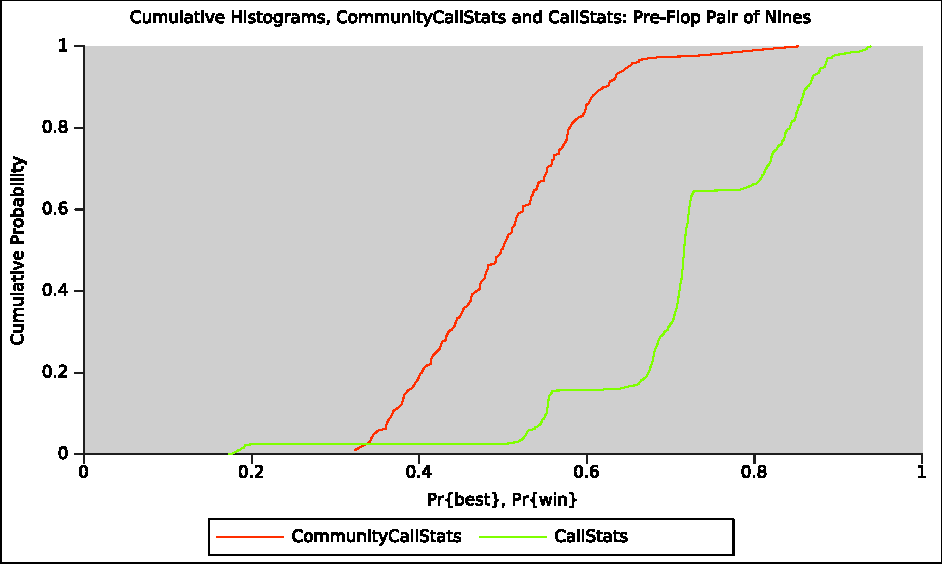
\includegraphics[width=0.8\textwidth]{cumu.pdf} 
 \end{center}
 \caption[Sample Cumulative Histograms]{The pre-flop CommunityCallStats cumulative histogram and the pre-flop CallStats histogram of a player holding a pair of nines. Notice from CommunityCallStats that the maximum $\mathrm{Pr\{win\}}$ of any pre-flop hole cards is about 85\% (pair of aces), but depending on the opponent's hand, it's possible for your pair of nines' $\mathrm{Pr\{win\}}$ to be as high as 94\% }
 \label{fig:Cumu}
\end{figure}


%Finally, since \texttt{CommunityCallStats} is almost completely independent of which hole cards a player holds, 
%Note that a single master \texttt{CommunityCallStats} can be generated as soon as the community cards are known, and the results can be efficiently shared between multiple poker bots running in the same process.
%This is not the case for \texttt{CallStats} or \texttt{WinStats}.
%The master \texttt{CommunityCallStats} for the current community are accessible through \texttt{HoldemArena::communityBuffer}.



\subsection{WinStats Histogram}
\label{sec:WinStats}

The \texttt{WinStats} histogram provides a sense how a set of community cards ``feels'' to a poker player.
To compute \texttt{WinStats}, iterate over all possible immediately upcoming community cards.
Here, immediate means the cards that can be dealt before the next betting round takes place.
For each possible combination of upcoming community cards, calculate how the player's average $\mathrm{Pr\{win\}}$ changes.

Most often, measures of spread and skew of $\mathrm{Pr\{win\}}$ across the various upcoming community cards create a quantitative description of ``bluffing hands'' and ``drawing hands''.
If the spread/variance of $\mathrm{Pr\{win\}}$ across all possible combinations of upcoming community cards is high, a player's position is relatively uncertain, and it may be safer to try to win the hand by bluffing than to work the game into a showdown.
If more of the upcoming community card combinations will worsen $\mathrm{Pr\{win\}}$ than improve it, the player should try to keep the betting low and wait to see if he/she will ``catch'' any of the few cards that will greatly improve his/her hand.
\texttt{WinStats} data is used more heuristically, whereas \texttt{CallStats} and \texttt{CommunityCallStats} are used more for purely probabilistic calculations.
In all cases, information from \texttt{WinStats} never overpowers the fundamental mathematics of making good poker decisions, but is used to add distinct ``personalities'' and ``playing styles'', each of which may be best suited to countering specific opponents.


\section{Value of Hole Cards}

%This section describes the definitions of $\mathrm{Pr\{win\}}$ and $\mathrm{Pr\{best\}}$ in more detail.


\subsection{Showdown Win Percentage}
\label{sec:Mean}
The mean of \texttt{WinStats} or the expectation of \texttt{CallStats} both provide $\mathrm{Pr\{win\}}$, the average chance of winning in a showdown against one opponent.
As mentioned in Section~\ref{sec:Approximations}, this measurement is extended to the $N$ opponent case by with the following approximations:
\[
\mathrm{Pr\{win all\}} = \prod_{\mathrm{opponents}} \mathrm{Pr\{win one\}} \approx \left( \mathrm{Pr\{win one\}} \right)^N
\]


\subsection{Best Hand Percentage}
\label{sec:Rank}
Once $\mathrm{Pr\{win\}}$ is known, \texttt{CommunityCallStats} can be used to calculate the probability of having a hand with a better chance of winning than $\mathrm{Pr\{win\}}$.
This is the hand's ``rank'' and represents the probability $\mathrm{Pr\{best\}}$ of having the better hand against one opponent.
$\mathrm{Pr\{best\}}$ is then extended to multiple opponents in the same way as $\mathrm{Pr\{win\}}$.


\section{Expected Utility}

%This section describes the relationships that define $\mathrm{E[callers}_x]$, $\mathrm{Pr\{push}_x\}$, and $\mathrm{Pr\{raised}_y\}$.
%The \texttt{ExactCallBluffD} class implements the general computation of $\mathrm{E[callers}_x]$, $\mathrm{Pr\{push}_x\}$, and $\mathrm{Pr\{raised}_y\}$.

\subsection{Showdown Utility}
\label{sec:Utility}
The $\mathrm{E[callers}_x]$, $\mathrm{Pr\{push}_x\}$, and $\mathrm{Pr\{raised}_y\}$ variables, in a sense, predict how your opponents will act.
In order to estimate another player's behaviour, we assume they will choose the action that has the highest utility.
As such, it is necessary to define a notion of utility.

The utility of a given hand acts as a measure of its worth.
If the outcome of betting a specific fraction of your bankroll on a certain scenario is random and independent, then in the long run the expectation of making the bet many times reduces to the geometric mean~\cite{KellyCriterion} of the outcomes.
If it is difficult or impossible to make the bet a large number of times, an arithmetic mean (or independent chip model~\cite{ICMmag2007} when the payout structure of a tournament is known) is more suitable.
For small bet of size $f$ that would occur many times throughout the course of a game, the total utility of making $N$ bets is:
\[
U = \left( \left( 1 + v_{\mathrm{win}} \left( f \right) \right)^{N_w} \left( 1 - v_{\mathrm{loss}} \left( f \right) \right)^{N_l} \right) \cdot B
\]
Here, the bet size $f$ is a fraction of the bankroll $B$, $N_w$ is the number of wins that occurred during the $N$ bets, and similarly $N_l$ is the number of losses.
$N = N_w + N_l$, $v_{\mathrm{win}} \left( f \right)$ is the payoff for winning the bet, and $v_{\mathrm{loss}} \left( f \right)$ is the price of making the bet (both are functions of the bet fraction $f$).
As $N \to \infty$, the incremental gain of each bet is simply the geometric mean of outcomes weighted by their probabilities, and extends easily to include the various split-pot situations, etc.
%The complete showdown gain model 

For large bets such as all-in calls that cannot be approximated using $N \to \infty$, a suitable short-term expectation of utility is the arithmetic mean equivalent:
\[
U = \left[ \left( 1 + v_{\mathrm{win}} \left( f \right) \right) \cdot N_w + \left( 1 - v_{\mathrm{loss}} \left( f \right) \right) \cdot N_l \right] \cdot B
\]

In all cases, $v_{\mathrm{win}} \left( f \right)$ is also a function of $\mathrm{E[callers}_x]$.
The computation of showdown utilities is implemented in the \texttt{GainModel} class for the geometric mean case, and the \texttt{GainModelNoRisk} derived class for the arithmetic mean case.



\subsection{Opportunity Cost of Folding}
\label{sec:FoldEquity}
Although the most obvious measure of utility is to consider the outcome of a showdown, it is possible to win chips in other ways as well.
If you make a bet large enough, you will force your opponents to fold, winning all of the chips in the pot.
This is known as pushing out your opponents, and has it's own associated utility.
In the reverse perspective, this concept becomes the opportunity cost of folding.

When facing a large bet $b$, you always have the option to either fold or play.
Often, it is more favourable to wait until the same opportunity arises again in the future, especially if it is likely for you to have better cards then.
Across $n$ situations facing the same bet, in your best opportunity to win out of those $n$ situation, you are likely have on average one of the $\frac{1}{n}^{\mathrm{th}}$ best hands.
From the rank ($\frac{1}{n}^{\mathrm{th}}$) of the hand and \texttt{CommunityCallStats}, its corresponding probability of winning ($p_{\mathrm{delayed}}(n)$, a function of $n$) can be obtained.
By waiting one hand (waiting until the same opportunity arises again) before playing, you will sacrifice whatever chips you have already committed to the pot in previous bets leading up to this one: $C_{committed}$.
By waiting $n$ opportunities before playing, you will sacrifice $n C_{committed}$.
However, you will improve your probability of winning to $p_{\mathrm{delayed}}(n)$.
Therefore, it is possible to win a total pot of $b-n C_{committed}$ with probability $p_{\mathrm{delayed}}(n)$, by folding now and expecting to wait an average of $n$ hands before calling.
For sufficiently large $b$ and a suitable \texttt{CommunityCallStats} histogram, it is advantageous to call from a better situation by folding now.

If \texttt{CommunityCallStats} is differentiable, for any given situation and bet faced, it is possible to solve for the optimal $n$ that maximizes the final expected utility.
Any money still lost in the maximum expected utility is the opportunity cost of folding, which in most cases is better than the cost of playing with a weak hand.

The computation of $n$ that optimizes the expectation of winning $b-n C_{committed}$ with probability $p_{\mathrm{delayed}}(n)$ can be achieved through any variety of unimodal function optimization techniques.
The expectation of the potential profit to be gained by folding against a bet that is too large is the ``FoldGain'' of a situation.
The \texttt{FoldGainModel} class implements these concepts.

\subsubsection{RiskLoss}
\label{sec:RiskLoss}
The ``opportunity cost of folding'' formula can also be applied from the perspective of the raiser, rather than the folder, in a sort of ``opportunity cost of raising'' heuristic.
The reverse application of the formula is implemented in a function called ``RiskLoss''.
This ``RiskLoss'' heuristic reports a loss (negative value) if your bet is large enough for the average opponent to profit (opportunity) by folding and waiting for a better hand.
%RiskLoss is computed by setting $C_{committed}$ to the average contribution to the pot by active players
Since making a small bet does not allow an average opponent to profit via his/her opportunity cost of folding, your ``RiskLoss'' remains zero as long as your bet is sufficiently small compared to an average opponent's opportunity.
The value returned by the RiskLoss function is used as a deterrent for raising too high.


\section{Opponent Modelling}

The following sections describe the approach used to estimate $\mathrm{E[callers]}$, $\mathrm{Pr\{push\}}$, and $\mathrm{Pr\{raise\}}$.
The computation of $\mathrm{E[callers]}$ and $\mathrm{Pr\{raise\}}$ is implemented in the \texttt{ExactCallD::query} function.
The computation of $\mathrm{Pr\{push\}}$ is implemented in the \texttt{ExactCallBluffD::query} function.

\subsection{Number of Callers}
\label{sec:Callers}
It is assumed that an opponent will only fold if the utility of his/her hand is too low to be worth playing.
For the purposes of computing $\mathrm{E[callers}_x]$, the geometric utility function is used, offset by the opportunity cost of folding.
The utility of a hand is a function of $w$, the percentage chance of winning in a showdown.
The utility function is more or less monotonic in $w$ and so there is a $w_{\mathrm{threshold}}$ for which the utility exactly zero.
$w_{\mathrm{threshold}}$ can be computed numerically using any variety of root-finding methodologies.
Depending on how well the opponent knows what hand you have, either the \texttt{CallStats} or \texttt{CommunityCallStats} (or a combination therefrom) histogram can be used to look up what percentage of hands have a chance to win greater than $w_{\mathrm{threshold}}$.
This is the fraction of opponents that are likely to play (call or raise).


Computing the total $\mathrm{E[callers}_x]$ for all opponents is not linear.
If the first opponent calls your bet, there is more money in the pot and more incentive for the next opponent to call.
A straightforward method of estimating $\mathrm{E[callers]}$ is to assume that each opponent will add $\mathrm{E[call]} = x \cdot \mathrm{Pr\{play\}}$ to the pot.
That amount is added to the pot, and is included in the calculation of $\mathrm{Pr\{play\}}$ for the next opponent.
Although opponents cannot generally call a fraction of the best, this provides a simple estimation of the aggregate call amount made by all opponents.
For each opponent, $\mathrm{Pr\{play\}}$ is the probability of that opponent calling or raising, and is solved numerically using the utility function described above.
If the total $\mathrm{E[callers}_x]$ turns out to be less than the bet to call, it is rounded up to avoid the case of having less than one call.
The value of $\mathrm{E[callers}_x]$ is not relevant if all opponents fold, and in practise, usually only one or two opponents make it to the showdown, so the accuracy of this estimate is acceptable.
For very easy calls over a large number of players, $\mathrm{E[callers}_x]$ will still sum to a large number of callers, and in more usual circumstances, $\mathrm{E[callers}_x]$ is generally between $x$ and $2x$.


\subsection{Pushes}
\label{sec:Push}
There is always a chance of making a bet large enough to push all of your opponents into folding.
If no opponents choose to play your bet, they will all fold and you win whatever is in the pot.
This is known as pushing out your opponents, and only occurs if nobody is willing to call (or raise) your bet.

We first let $\mathrm{Pr\{play\}}$ be the probability that any opponent decides to play (i.e. decides not to fold).
The probability $\mathrm{Pr\{play\}}$ is computed with almost the same approach as for $\mathrm{E[callers}_x]$, with a few minor distinctions.
Firstly, in general, when your bet is so large that all players will decide to fold, the bet size will fall in the category of arithmetic mean utility functions rather than geometric mean utility functions.
Secondly, making a large bet gives more away about the hand that you hold, and therefore, in the spirit of the minimax/Nash equilibrium approaches, more weight is deliberately given to the worse of \texttt{CallStats} or \texttt{CommunityCallStats} when looking up $\mathrm{Pr\{play\}}$ from the computed $w_{\mathrm{threshold}}$.
Once $\mathrm{Pr\{play\}}$ is known for each player, the product $\mathrm{Pr\{push\}} = \prod_{\mathrm{opponents}} \left( 1 - \mathrm{Pr\{play\}} \right)$ is the total probability of winning the pot due to opponent folds.
See \textbf{Figure~\ref{fig:Pr}} for example $\mathrm{Pr\{push\}}$ behaviour plotted using real simulation data.


\subsection{Raises}
\label{sec:Raises}
Your opponent may choose to raise rather than call, forcing you to make a new decision.
An opponent is motivated to raise rather than call if he/she can win more money by making you call a larger amount.
However, if your opponent's bet is too large, it becomes profitable for you to fold due to `FoldGain'.

Furthermore, it may not always be profitable in a showdown for the opponent to have called or raised your bet.
Your opponent may prefer to raise with the hope that you fold, rather than being the one to fold himself/herself.
Therefore, an opponent should choose to raise whenever the expected value of raising outweighs the expected value of both calling or folding, with all opportunity costs considered.

The utility of an opponent's hand is a function of both $w$, the percentage chance of winning in a showdown, and $b$, the size of bet that he/she decides to make.
For raises, we apply the geometric mean model to the opponent's utility $U(w,b)$.
The resulting inequality describes the condition required for an opponent to raise:
\[
\mathrm{Utility\:of\:raising} + RiskLoss > max\{\mathrm{Utility\:of\:calling}, FoldGain\}
\]
Rearranging,
\[
U(w,b_{\mathrm{raiseTo}}) + RiskLoss - max\{U(w,b_{\mathrm{call}}), FoldGain\} > 0
\]
The left hand side of the inequality is implemented in the \texttt{FacedOddsRaiseGeom} class, and is a function of $w$.
Let $w_r$ be the value at $w$ at the boundary of the inequality (i.e. the value that causes the left hand side of the equation to be zero).
This way, $w_r$ represents the minimum chance to win that opponent would desire in order to choose to raise.
The value of $w_r$ can be computed using any standard 1-D root finding technique.
Then, \texttt{CommunityCallStats} can be used to look up the fraction of opponents that are likely to have a hand $w_r$ good or better, which in turn, is the probability that a single opponent will have a hand good enough to raise you to $b_{\mathrm{raise}}$.
For any given $b_{\mathrm{raise}}$, the $w_r$ and therefore the probability of raising ($\mathrm{Pr\{raise\}}$) for a single opponent can be computed.
Extending to multiple opponents:
\[
\mathrm{Pr\{anyOpponentRaise\}} = 1 - \prod_{\mathrm{opponents}} \left( 1 - \mathrm{Pr\{raise\}} \right)
\]


In general, we will omit RiskLoss from the inequality if $max\{U(w,b_call), FoldGain\} = U(w,b_call)$, that is, we do not consider RiskLoss when the utility of calling is more significant than FoldGain.
The reason for this is because RiskLoss is meant to act as a deterrent for raising too high.
When any player wins money by raising in a situation where folding is safer than calling, it is generally because that player will force everybody else to fold -- not because the player had good cards.
The bet most likely to force everybody else to fold is an all-in bet.
However, betting all-in provides everybody else with an implicit FoldGain of their own, so RiskLoss is used to offset FoldGain for such bets that are so large that they become profitable to others.
On the other hand, when a player has good cards, the utility of calling is higher than the utility of folding.
Then, the decision of whether to call or raise is simply about adding more money to the showdown or not, and the RiskLoss deterrent isn't needed.
Furthermore, \texttt{FacedOddsRaiseGeom} currently does not explicitly consider the expected utility due to the possibility of everybody else folding, and the removal of RiskLoss plays that role somewhat in the comparison between the utility of raising vs. calling.
See \textbf{Figure~\ref{fig:Pr}} for example $\mathrm{Pr\{raise\}}$ behaviour plotted using real simulation data.

\begin{figure}[htb]
 \begin{center}
      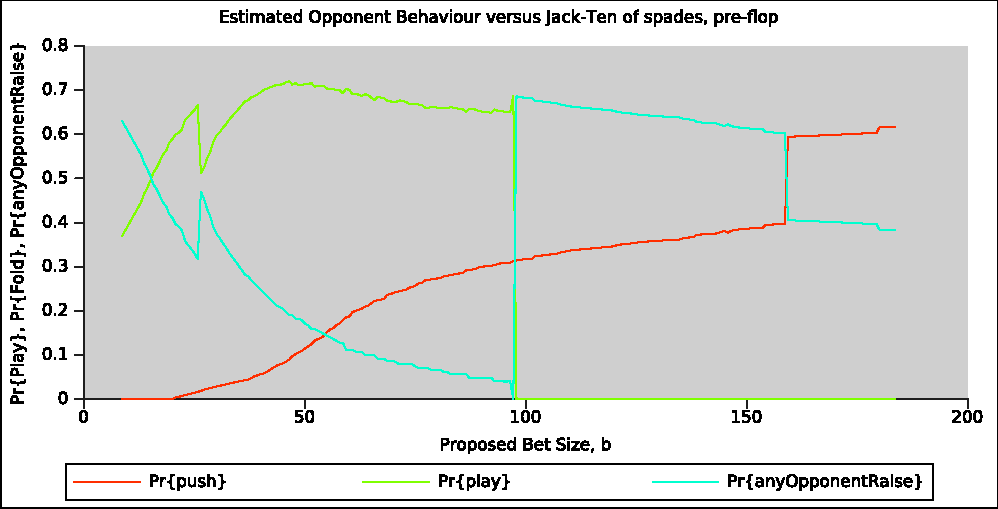
\includegraphics[width=0.8\textwidth]{pr.pdf} 
 \end{center}
 \caption[$\mathrm{Pr\{fold\}}$, $\mathrm{Pr\{play\}}$, and $\mathrm{Pr\{raise\}}$]{ $\mathrm{Pr\{fold\}}$, $\mathrm{Pr\{play\}}$, and $\mathrm{Pr\{raise\}}$ are estimated in a preflop situation. Notice the jump from 70\% play to 70\% push at a bet size of about half of the remaining chips. Once a bet is that big, if your opponent has any interest in playing he/she may as well re-raise all in. The smaller jump at about 30 chips is a similar situation with a different opponent who has only a small number of chips remaining.}
 \label{fig:Pr}
\end{figure}

%\clearpage
